 %\documentclass[11pt]{article}
\documentclass{llncs}
\usepackage[boxed,vlined]{algorithm2e}
% \usepackage{epsf}
\usepackage{graphics}
%\usepackage{epsfig}


\title{RBO Protocol:
Broadcasting Huge Databases for Tiny Receivers%\thanks{
% This work has been supported by MNiSW grant N N206 1842 33
% }
%\thanks{
% This work has been  supported by the ICT Programme of
% the European Union under contract number FP7-215270 (FRONTS)
%}
}
\author{Marcin Kik\\
\email{ {Marcin.Kik@pwr.wroc.pl}}\\
\institute{{Institute of Mathematics and Computer Science},\\
           {Wroc\l aw University of Technology}\\
           Wybrze\.ze Wyspia\'nskiego 27, 50-370 Wroc\l aw, Poland}
}


\SetKw{KwProcedure}{procedure}
\SetKw{KwDownto}{downto}
\SetKw{KwFunction}{function}
\SetKw{KwReturn}{return}

\newcommand{\irmo}{\mbox{\sf irmo}}
\newcommand{\lbo}{\mbox{\sf lbo}}
\newcommand{\lev}{\mbox{\sf lev}}
\newcommand{\bo}{\mbox{\sf bo}} 
\newcommand{\rbo}{\mbox{\sf rbo}}
\newcommand{\ident}{\mbox{\sf ident}}
\newcommand{\minR}{\mbox{\sf minR}}
\newcommand{\maxR}{\mbox{\sf maxR}}
\newcommand{\idx}{\mbox{\sf idx}}
\newcommand{\key}{\mbox{\sf key}}



\pagestyle{plain} %%% Wykomentowac w CAMERA_READY 

\begin{document}


\maketitle % llncs

% \thispagestyle{plain} %%%%  

\begin{abstract}
RBO is a protocol for a powerful sender and tiny (battery powered) receivers.
The sender repeatedly broadcasts a sequence of many (possibly millions) of messages,
while each receiver is interested in reception of a specific message within this
sequence.
The transmission is arranged so that the receiver can wake up in arbitrary moment and find
 the nearest transmission of its searched message.  
Even if it does not know the position of the message in the sequence,
it needs only
to receive a small number of other messages to locate it properly.
Thus it can save energy by keeping the radio switched off most of the time.
We show that bit-reversal permutation has ``recursive bisection properties''
and, as a consequence,
RBO can be implemented very efficiently 
with only constant number of $\lceil\log_2 n\rceil$-bit variables,
where $n$ is the total number of messages in the sequence. 
The total number of the required receptions is at most $2\lceil\log_2 n\rceil+2$ 
in the model with perfect synchronization.
The basic procedure of RBO 
(computation of the time slot for the next required reception)
requires only $O(\log^3 n)$ bit-wise operations.
We propose implementation mechanisms 
for realistic model (with imperfect synchronization),
for operating systems (such as e.g. TinyOS).
 
   

\end{abstract}


\section{Introduction}
RBO is a protocol for a powerful sender and tiny (battery powered) receivers.
The sender repeatedly broadcasts a sequence of many (possibly millions) of messages.
Each message is labeled by a {\em key}.
At arbitrary time moment the user of RBO 
(i.e. some application running on the receiver device)
may ask the RBO module to receive a message with some specified key.
Since then, the task of the RBO module is to receive the nearest transmission 
of the  message labeled with this key and deliver this message to the user.
The simplest strategy would be keeping the radio switched on and listen to all
messages until the searched one is received.
However, radio consumes a lot of energy while it is switched on and the receiver 
device has a limited energy source (i.e. battery).
If the whole sequence contains millions of messages, then
we may need to wait many hours until the searched message is transmitted.
Therefore we need a strategy that minimizes the total radio working time
and does receive the nearest transmission of the searched message. 
Transmitting large database for battery powered
receivers has been considered in 
\cite{DBLP:conf/sigmod/ImielinskiVB94},
\cite{DBLP:conf/edbt/ImielinskiVB94},
and 
\cite{DBLP:journals/tkde/ImielinskiVB97}.
They proposed techniques based on hashing and inclusion of
indexing informations in data stream that let the receiver 
energetically efficient searching for data. 

The RBO protocol is based on a simple ranking algorithm
for single hop radio network proposed in \cite{DBLP:conf/adhoc-now/Kik08}.
The sender sorts the messages by their keys and then permutes them by a special permutation
(called {\em recursive bisection ordering} or {\em $rbo$}).
Such sequence is periodically broadcast.
The receivers' RBO protocol 
keeps an interval $[minR, maxR]$ of possible ranks of the searched key 
in the transmitted sequence.
Initially $[minR, maxR]=[0, n-1]$, where $n$ is the length of the sequence.
RBO tries to receive {\em only} the messages with the keys ranked in $[minR, maxR]$.
Each such message is either the searched one
or it can be used for further updating (shrinking) of the interval.
It has been shown in \cite{DBLP:conf/adhoc-now/Kik08} that 
% only logarithmic number of 
no more than $4\lg_2 n$
messages are required to locate the rank of the
key in the sequence if the sequence is retransmitted in rounds,
even when the search is started in arbitrary time slot.

We use $rbo'$ -- slightly modified version of the $rbo$ permutation from\cite{DBLP:conf/adhoc-now/Kik08}:
By keeping zero as the fixed point in the definition, we
obtain a permutation $rbo'$ that is actually {\em bit-reversal} permutation
(famous for its application in FFT \cite{CormenLR89}).
This enables very efficient and simple implementation
of the functions needed by the RBO protocol.
Hence, RBO can be implemented on very weak devices with tiny memory
resources (such as e.g. sensors).

In section \ref{nextSlotIn-section} we propose simple and efficient 
% (polylogarithmic time)
 algorithm
for computing next time slot that should be received by the receiver.
The algorithm enables 
computations for very long sequences of messages (possibly many millions or more) 
even on very weak processors. It requires $O(\lg^3 n)$ bit-wise operations.

In section \ref{reliable-efficiency-section}
we show precise upper bound on
the number of necessary receptions required 
to reach the searched message.
The bound is $2\lceil\lg_2 n\rceil+2$.
(Due to the simpler permutation and more detailed proof,
this bound is lower than the one in \cite{DBLP:conf/adhoc-now/Kik08}.)
We show an example, when $2\lceil\lg_2 n\rceil-1$ receptions are required.

In section \ref{implementation-section}
we propose the implementation of the protocol on real devices.
A prototype of the protocol with a simple demonstration application 
has been implemented in Java language
and is available at \cite{RBO-WWW}.
This implementation is designed to be 
easily transformable to TinyOS (\cite{TinyOSProgramming}, \cite{TinyOS-WWW}):
The required modules of TinyOS, hardware components and radio channel
has been modelled by appropriate objects.
RBO protocol offers split-phase interface to the user.
The user issues a command to find a message with given key and,
after some time is signalled the call-back with the results
of the search.
In the meantime RBO switches the radio receiver on and off:
on the one hand -- to save energy, on the other hand -- 
to ensure the reception of all the messages required for the search.
Also the basic protocol functions have been implemented with any recursion
removed (to save memory) and optimized up to the bitwise operations. 
 

Another application of the RBO can be centralized channel access
control for upload transmissions (e.g. for overcrowded channel): 
The base station broadcasts only the headers,
while the rest of the time slot can be used for
transmission by the (unique) owner of the key from the header.

\section{Preliminaries}
 
We assume that the length of the transmitted sequence is $n=2^k$, for
some positive integer $k$.
(If the actual number of messages is not power of two, then
we can double some of them to obtain a sequence of length $2^k$.)


Let $bs_k$ be a permutation of $\{0,\ldots,2^k-1\}$ defined as follows:
\begin{itemize}
\item for $k=0$, ${bs}_k (x)=0$, and,
\item for $k>0$, ${bs}_{k } (x)  =  (1-(x\bmod 2))\cdot {bs}_{k-1} (\lfloor x / 2 \rfloor) 
                            + (x\bmod 2) \cdot (2^{k-1} + \lfloor x / 2 \rfloor)$.
\end{itemize}
Even ranks, permuted by $bs_{k-1}$, are placed before 
the odd ones -- the {\em leaves} of {\em binary search tree}.
The graph of this permutation (black points) is shown as the leftmost one on Figure~\ref{fig-trees}.
On the graphs, 
the axis of domain (corresponding to {\em ranks}) is directed rightwards, 
while the axis of the range (corresponding to {\em time}) is directed downwards.
The line segments form a {\em binary search tree}.
A node $(x,y)$ on the graph is on the level $\lceil\lg_2(y+1)\rceil$ in the tree. 
If sender transmits a sorted sequence of length $2^k$ permuted by $bs_k$
and the receiver starts listening in time slot zero, then it needs to 
receive no more than $k$ keys to locate its search key.
However, if the receiver starts at arbitrary time, then it may be forced to 
receive many messages.
(Consider the case, when the receiver starts in time slot $2^{k-1}$ and the searched key
is greater than all the keys of the sequence.)
In {\em binary search} it is essential, 
that all the nodes from one level precede all the nodes from the next level.
However, the ordering of the nodes within each level may be arbitrary.  
Hence, instead of $bs_k$ we use $rbo'_k$ defined as follows:
\begin{itemize}
\item for $k=0$,  ${rbo'}_k(x) =  0$, and,
\item for $k>0$,   ${rbo'}_{k}(x)  =  {rbo'}_{k-1} (\lfloor x / 2 \rfloor) 
                         + (x\bmod 2) \cdot 2^{k-1}$.
\end{itemize}
Here each level $l$ (of size $\lceil 2^{l-1}\rceil$) is {\em recursively permuted} by $rbo'_{l-1}$.

Let $revBits_k$ denote a {\em $k$-bit-reversal permutation}:
  for $0 \le x < 2^k$,  
  $revBits_k (x) = \sum_{i = 0}^{k -1} 2^i \cdot x_{k - 1 - i}$, where $x_i = \lfloor x / 2^i\rfloor \bmod 2$.
By unfolding the recursion on $rbo'_k$,
you may notice that:
% \begin{lemma}
  $rbo'_k = revBits_k (= (rbo'_k)^{- 1})$. 
% \end{lemma}
However, the recursive definition of $rbo'$ shows its essential property:
The nodes within level $l$ of the binary search tree form a binary search tree and
the same holds for the sub-levels of the level.
The binary search tree for $rbo'_5=revBits_5$ is shown on the middle graph on Figure~\ref{fig-trees},
while the trees for its levels (the first level of recursion) are shown on the rightmost graph.


\begin{figure}
\centering{\resizebox{!}{35mm}{
    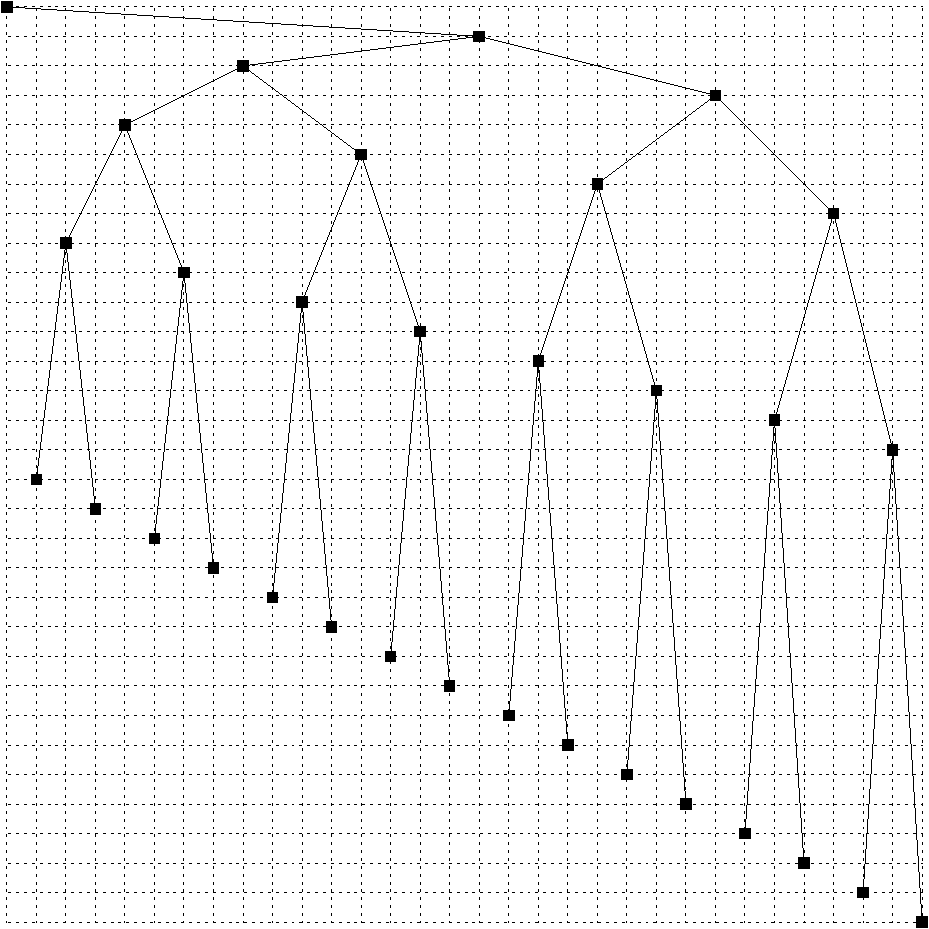
\includegraphics{bs5tree.pdf} \hspace{2cm} 
    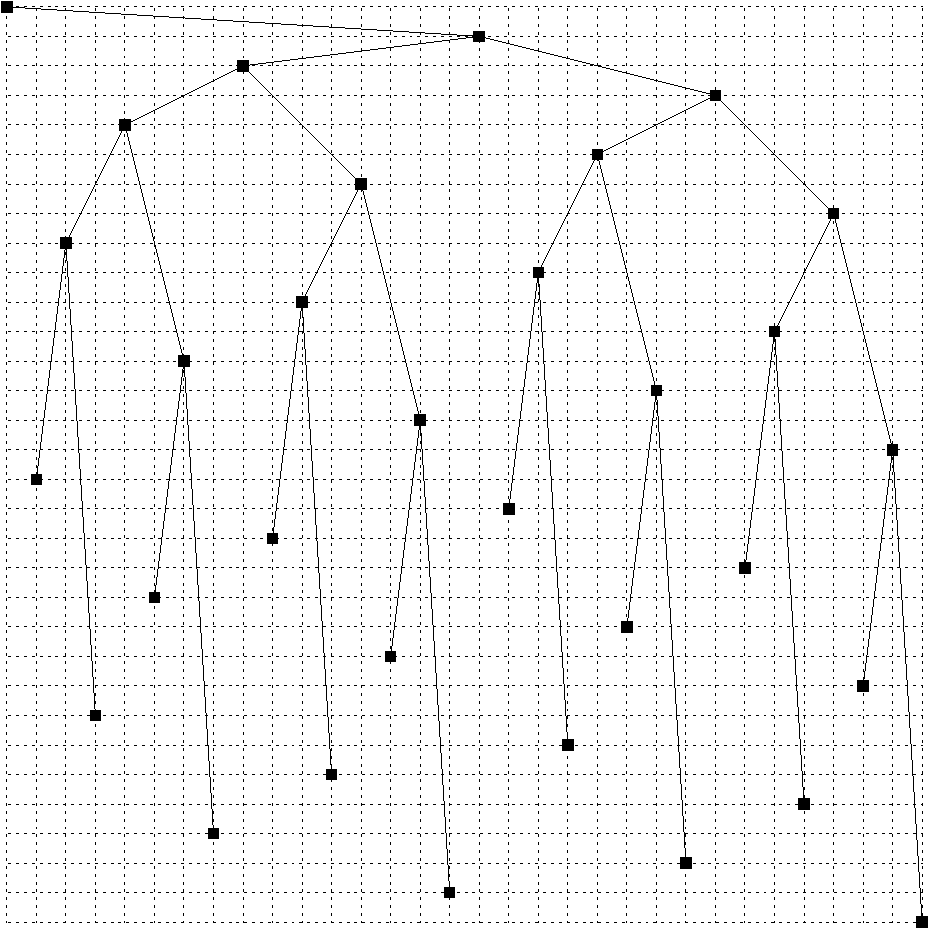
\includegraphics{revBits5tree.pdf} \hspace{2cm}
    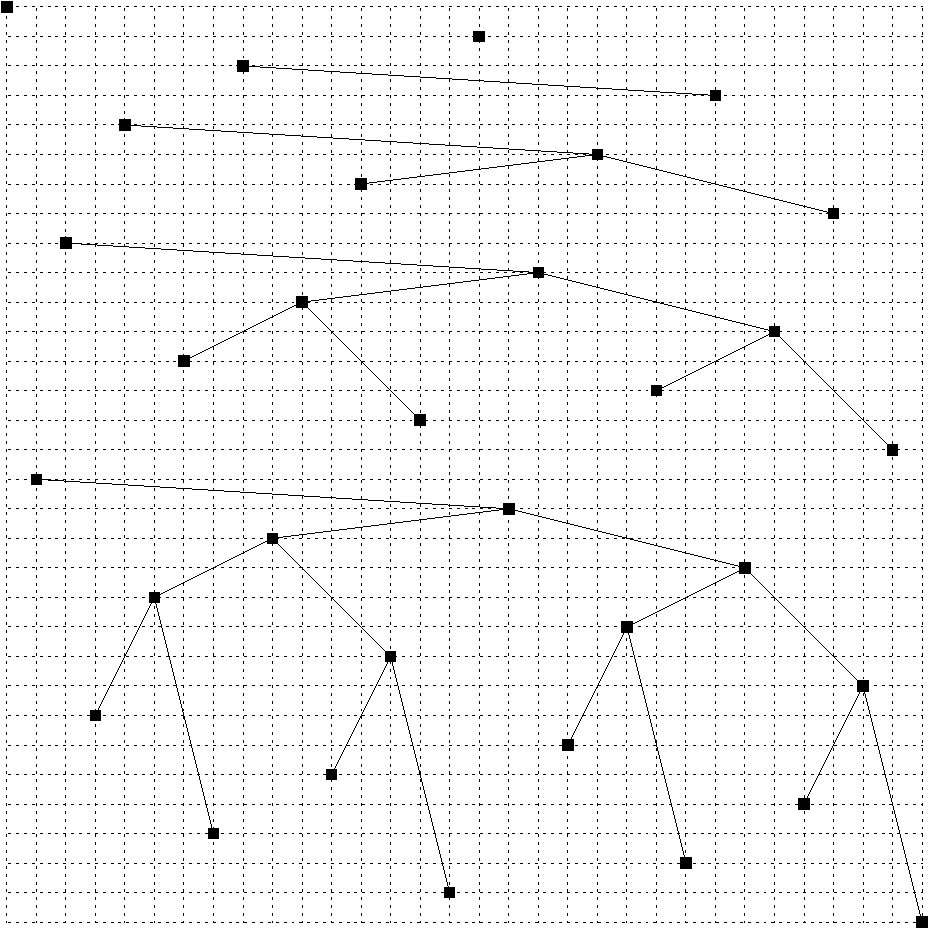
\includegraphics{revBits5-1trees.pdf} \hspace{2cm}
  }
}
\caption{The graphs of permutations: $bs_5$ (leftmost one),  $rbo_5=revBits_5$ (remaining two).\label{fig-trees}}
\end{figure}

The domain of the $revBits_k$ corresponds to {\em ranks}, while its range corresponds to {\em time slots}.
The {\em binary search tree} of $revBits_k$ has $k+1$ {\em levels}: $0$,$\ldots$,$k$.
By the {\em level} of the {\em time slot} $t$ we mean $\lceil \lg_2 (t+1)\rceil$,
and by the {\em level} of the {\em rank} $x$ we mean $\lceil \lg_2 (revBits_k(x)+1)\rceil$.
For each rank $x$ on level $l$, $0\le x<2^k$ and $x=2^{k-l}+i_x\cdot 2^{k-l+1}$, for some integer $i_x$
called {\em coordinate of $x$ within level $l$}.
(Note that $i_x=\lfloor x/2^{k-l+1}\rfloor$.)

 




\section{Computation of $nextSlotIn$}\label{nextSlotIn-section}

The most important function used by the RBO protocol is $nextSlotIn_k$ defined,
for $0\le t<2^k$, $0\le r_1\le r_2<2^k$, as follows:
$$
nextSlotIn_k(t, r_1, r_2)=
$$
$$
\left(t+\min\{d>0 : r1\le revBits_k( (t+d)\bmod 2^k   ) \le r_2\}\right) \bmod 2^k 
$$
(I.e. the number of the next slot after $t$ with rank in $[r_1,r_2]$.)
Efficient computation of this function reduces the 
time and the energy used by the processor of the receiver.
If $2^k/(r_2-r_1)$ is not too large (e.g. below one hundred)
then the distance between consecutive elements of $revBits([r_1,r_2])$ 
is not large and we may {\em naively} check sequentially the slots $t_0$, $t_0+1$, $\ldots$ (modulo $2^k$), 
starting from $t_0=(t+1)\bmod 2^k$. 
Otherwise, if $r_2-r_1$ is a small number, then we may apply {\em reverse} search, 
among time slots $revBits(r_1)$, $\ldots$, $revBits(r_2)$, 
for the nearest successor of $t$.
We propose poly-logarithmic time computation 
of $nextSlotIn$, 
that should be applied when both
$2^k/(r_2-r_1)$ and $r_2-r_1$ are large.
%If both $2^k/(r_2-r_1)$ and $r_2-r_1$ are large then we may apply poly-logarithmic time computation 
% of $nextSlotIn$.
The implementation of this algorithm in programming language can be found in \cite{RBO-WWW} or Appendix~\ref{Rbo-Java}.
Here we describe its idea and a more intuitive pseudo-code.
First let us see how to compute the (globally)  minimal time slot $t$,
such that $revBits(t)\in [r_1,r_2]$.
Let $minRevBits_k(r_1,r_2)=\min revBits_k(\{x\, |\, r_1\le x\le r_2\})$.
Note that if $x$ is (the rank of) the node of the binary search tree,
then the left (respectively, right) child of $x$ is $x_l=x-2^{k-l-1}$ 
(respectively, $x_r=x+2^{k-l-1}$), where $l$ is the
level of $x$.
We can compute $minRevBits_k$ %, in time $O(k)$,
by following the the path on binary search tree until
we enter the interval $[r_1,r_2]$ (see Algorithm~\ref{minRevBits} or Appendix~\ref{Rbo-Java}).
\begin{algorithm}
  \KwFunction $minRevBits_k( r_1, r_2 )$\\
  $x\gets 0$; $s\gets 2^{k-1}$;\\
  \While{$x<r_1$ or $x>r_2$}
      {
        \lIf{$x<r_1$}
            {
              $x\gets x+s$
            }
            \lElse 
                {
                  $x\gets x-s$
                }\\
                $s\gets s/2$;
      }
      \KwReturn $revBits(x)$;
      \caption{Computing $minRevBits$\label{minRevBits}}
\end{algorithm}
By symmetry of $revBits_k$, we have 
that $maxRevBits_k(r_1,r_2)=\max revBits_k(\{x\, |\, r_1\le x\le r_2\})$ is equal to
$2^k-minRevBits_k(2^k-r_2, 2^k-r_1)$.
(See Appendix~\ref{Rbo-Java}).

Here is the outline of our algorithm for computing $nextSlotIn_k(t, r_1,r_2)$:
\begin{enumerate}
\item
If $r_1<r_2$ then 
if $revBits_k(t)=r_1$, then $r_1\gets r_1+1$
else
if $revBits_k(t)=r_2$, then $r_2\gets r_2-1$.
(I.e. remove $revBits_k(t)$ if it is {\em only} one side of the interval.)


\item
If $r_1=r_2$ then {\bf return} $revBits_k(r_1)$. (There is no choice.)


\item 
Let $tFirst=minRevBits_k(r_1, r_2)$.
If $t<tFirst$ then {\bf return} $tFirst$.

\item 
Let $tLast=maxRevBits_k(r_1, r_2)$.
If $tLast\le t$ then {\bf return} $tFirst$. 
(The first slot ranked in $[r_1,r_2]$ in the next round of broadcasting.)

\item\label{find-level-step}
Find minimal level $l$, such that $l\ge \lceil\lg_2 (t+1)\rceil$ and
% $minL=\min \{x\ge r_1 \,|\, x=2^{k-l}+i\cdot 2^{k-l+1} \}$
$minL=\min \{i\,|\, 2^{k-l}+i\cdot 2^{k-l+1}\ge r_1 \}$
is not greater than
% $maxL=\max \{x\le r_2 \,|\,   x=2^{k-l}+i\cdot 2^{k-l+1} \}$.
$maxL=\max \{i \,|\,   2^{k-l}+i\cdot 2^{k-l+1}\le r_2 \}$.
Such $l$ is the first level (starting from the level of $t$) that
intersects  $\{r_1,\ldots,r_2\}$.
Then
$aboveL=2^{l-1}$ is the number of nodes above the level $l$
(and also the size of the level $l$) and
 $\{minL,\ldots,maxL\}$ 
are the coordinates  {\em within} the level $l$ of its intersection with $\{r_1,\ldots,r_2\}$. 
(Note that
$minL=\lceil (r_1-2^{k-l})/2^{k-l+1}\rceil = \lfloor (r_2+2^{k-l}-1)/2^{k-l+1}\rfloor$,
and $maxL= \lfloor (r_2-2^{k-l})/2^{k-l+1}\rfloor$.)

\item 
Let $tFirstL= minRevBits_{l-1}(minL, maxL)$
(first slot of the level $l$ ranked in $[minL, maxL]$).
If $t< aboveL+tFirstL$ then {\bf return} $aboveL+tFirstL$.

\item
Here $l$ is the level of $t$, since we did not return in previous step.
Let $tLastL= maxRevBits_{l-1}(minL, maxL)$.

\item\label{find-level-step1}
If $t\ge aboveL+tlastL$ then %(actually $t=aboveL+tlastL$)
we have to find the first slot in $[r_1,r_2]$ below the level $l$: 
  \begin{enumerate}
  \item\label{find-level-step1-substep}
  Find minimal level $l_1>l$, such that 
  $minL_1=\min \{i \,|\, 2^{k-l_1}+i\cdot 2^{k-l_1+1}\ge r_1 \}$
  is not greater than
  $maxL_1=\max \{i \,|\, 2^{k-l_1}+i\cdot 2^{k-l_1+1}\le r_2 \}$.
  Then
  $aboveL_1=2^{l_1-1}$ is the number of nodes above the level $l_1$
  % (and also the size of the level $l_1$) 
  and
  $minL_1$ and $maxL_1$ 
  are the coordinates {\em within} the level $l_1$. 

  \item 
  Let $tFirstL_1= minRevBits_{l_1-1}( minL_1, maxL_1)$. {\bf Return} $aboveL_1+tFirstL_1$.

  \end{enumerate}

\item 
Here $tFirstL\le t-aboveL <tLastL$ and we search within the level $l$ ({\em tail recursion}):
{\bf Return} $aboveL+nextSlotIn_{l-1}(t-aboveL, minL, maxL)$.

\end{enumerate}

The depth of the recursion is at most $k$, since each level has no more than 
a half of the nodes of the tree.
Step~\ref{find-level-step1-substep} is only on last recursion.
In step~\ref{find-level-step}, $t$ is above level $l$ only on last recursion.
Thus, the algorithm performs $O(k)$ {\em elementary} operations
such as $revBits$, $minRevBits$, $maxRevBits$ or arithmetic operations. 
Since each such operation  needs $O(k^2)$ bit operations,
the total cost is $O(\log^3 n)$ of bitwise operations.
% Many of the operations can be efficiently implemented using bitwise operators.
We replace {\em tail recursion}  by iterative version 
(see \cite{RBO-WWW} or Appendix~\ref{Rbo-Java}).
Thus RBO uses only constant number of $\lceil\log_2 n\rceil$-bit variables.




%%%%%%%%%%%%%%%%%%%%%%%%%%%%%%%%%%%%%%%%%%%%%%%%%%%%%%%%%%%%%%%%%%%%%%%%%%%%%%%%%
\section{Time and Energetic Efficiency}\label{reliable-efficiency-section}

\begin{theorem}\label{reliable-theorem}
Let $n=2^k$.
Let $\kappa_0$,$\ldots$,$\kappa_{n-1}$ be a sorted sequence of keys.
Let $\kappa$ be arbitrary searched key , 
let $t_0$ be arbitrary time slot, $0\le t_0<n$, and,
let $minR_0=0$ and $maxR_0=n-1$.
For $i\ge 0$, let $t_{i+1}= nextSlotIn(t_i, minR_i, maxR_i)$, and,
\begin{itemize}
\item
  if $\kappa<\kappa_{revBits(t_{i+1})}$ then $minR_{i+1}=minR_i$ and $maxR_{i+1}=revBits(t_{i+1})-1$,
  else
\item
  if $\kappa>\kappa_{revBits(t_{i+1})}$ then $minR_{i+1}=revBits(t_{i+1})+1$ and $maxR_{i+1}=maxR_i$,
  else 
\item
  $minR_{i+1}=minR_i$ and $maxR_{i+1}=maxR_i$.
\end{itemize}
Let $e=\min\{i>0 \,|\, minR_i\ge maxR_i \vee \kappa_{revBits(t_{i})}=\kappa\}$.
%Under the above assumptions we have:
We have:
\begin{enumerate}
\item\label{reliable-energy}
  % (bound on energy)
  $e\le 2\lg_2 n+2$, and
\item\label{reliable-time}
  % (bound on time.)
  % $t_e-t_0\le n$.
  $t_e$ is at most $n$ time slots after $t_0$.
\end{enumerate}
\end{theorem}
\begin{proof}
% The key observation is that arbitrary time slot is a root of a binary search tree
% defined on some recursion level.

Note that $t_1= (t_0+1)\bmod n$,
and $t_1$, $t_2$, $\ldots$, $t_e$ are the reception time slots 
required by the search for $\kappa$ 
started just before $t_1$. 
If $\kappa\in \{\kappa_0,\ldots,\kappa_{n-1}\}$,
then the sequence $(t_1,t_2,$ $\ldots$, $t_{e-1},t_e)$ is
a prefix of the sequence of time slots used for 
searching for some $\kappa'\not\in \{\kappa_0,\ldots,\kappa_{n-1}\}$
with the same rank as $\kappa$.
Therefore we consider only the case: $\kappa\not\in \{\kappa_0,\ldots,\kappa_{n-1}\}$.

Note that $\{ \kappa_{t_1}, \kappa_{(t_1+1)\bmod n},\ldots, \kappa_{(t_1+n-1)\bmod n}\}$
contains all the keys $\kappa_0$,$\ldots$,$\kappa_{n-1}$.
Hence, the bound on time (part~\ref{reliable-time}) is valid.

Now consider the part~\ref{reliable-energy} (the bound on energy).
Let $U$ denote the set of the (used) time slots $\{t_1,t_2,\ldots,t_{e-1},t_e\}$.
% Let $\alpha=(l_0,\ldots,l_i)$ be a sequence.
Let $()$ denote an empty sequence.
Let $\alpha_1\cdot\alpha_2$ denote the 
concatenation of sequences $\alpha_1$ and $\alpha_2$.
Let $|\alpha|$ denote the length of the sequence $\alpha$.
% and $last(\alpha)$ be the last element of $\alpha$).
For a decreasing sequence $\alpha$ of numbers from $\{0,\ldots,k\}$, 
we define $Y_\alpha$ as follows:
\begin{enumerate}
\item
  $Y_{()}=\{0,1,\ldots, n-1 \}$.

\item for $0\le l\le \lg_2 |Y_\alpha|$,
  $Y_{\alpha\cdot (l)}=\{ y\,|\, \lceil \lg_2(y-\min Y_\alpha+1)\rceil = l \}$.
  (Equivalently: 
   $Y_{\alpha\cdot (l)}=\{ y\,|\, \min Y_{\alpha}+\lfloor 2^{l-1}\rfloor \le y< \min Y_{\alpha}+2^l \}$.)
\end{enumerate}

Let $X_\alpha=revBits(Y_\alpha)$.
Note that:
\begin{lemma}\label{basic-lemma}
\begin{enumerate}
\item
  $Y_{\alpha\cdot (l)}$ (respectively, $X_{\alpha\cdot (l)}$)
  is the set of time slots (respectively, ranks) on the $l$th level of the binary search tree $Y_\alpha$.
\item
  $|Y_{\alpha\cdot(0)}|=|X_{\alpha\cdot(0)}|=1$ and,
  for $0<l\le \lg_2 |Y_\alpha| $, $|Y_{\alpha\cdot(l)}|=|X_{\alpha\cdot(l)}|=2^{l-1}$.
\item
  $Y_\alpha$ (respectively, $X_\alpha$) is
  a disjoint union of the sets $Y_{\alpha\cdot (l)}$ (respectively, $X_{\alpha\cdot (l)}$),
  where $0\le l\le \lg_2 |Y_\alpha|$. %=\lg_2 |X_\alpha|$.
\item\label{basic-minimum}
  $\min Y_{(l_0,l_1,\ldots,l_r)}=\sum_{i=0}^r \lfloor 2^{l_r-1}\rfloor$.
\end{enumerate}
\end{lemma}

Let $\beta$ be the shortest sequence, such that $\min Y_\beta= t_1$.
If $\beta=()$, then $t_1=0$ and we start binary search from the global root.
(Thus each of $t_1, \ldots, t_{e}$ is on distinct level and, hence, $e\le k+1$.)
Otherwise, % let $\beta=(l_0,\ldots,l_R)$.
let $\beta_0=\beta$ and, for $j\ge 0$, let $\beta_{j+1}$ be defined
as follows:
\begin{itemize}
\item 
  if $\beta_j=()$, then $\beta_{j+1}$ is not defined, 
  else
\item 
  if $\beta_j=\alpha\cdot (l',l, l-1,\ldots, l-m)$,
  where $l+1<l'$ and $m\ge 1$, 
  then $\beta_{j+1}=\alpha\cdot(l',l+1)$, 
  else
\item 
  if $\beta_j=(l,l-1,\ldots,l-m)$,
  where $l<k$ and  $m\ge 1$,
  then $\beta_{j+1}=(l+1)$, 
  else
\item 
  if $\beta_j=(k,k-1,\ldots,k-m)$,
  where $m\ge 0$,
  then $\beta_{j+1}=()$, 
  else
\item 
  $\beta_{j+1}=\alpha\cdot (l+1)$, 
  where $\beta_j=\alpha\cdot (l)$.

\end{itemize}
Let $last=\min\{j\,|\, \beta_j=()\}$.
For $0\le j\le last$,
if $\beta_j=\alpha\cdot(l)$, then let $f_j=l$,
else (i.e. when $\beta_j=()$) let $f_j=k+1$.
The following lemma follows directly from the definitions of $\beta_j$ and $last$.
\begin{lemma}\label{foot-increasing-lemma}
For $0\le j<last$, $f_j+1+|\beta_j|-|\beta_{j+1}|= f_{j+1}$ and $f_{last}= k+1$.
\end{lemma}
Note that $last\le k$, since $f_0\ge 0$, and $f_j<f_{j+1}$ (since $|\beta_j|\ge |\beta_{j+1}|$), 
and $f_0=0$ implies $|\beta_0|>1$.

Note that $(t_1,(t_1+1)\bmod n,$ $\ldots$ $, t_e)$ is a prefix of the sequence
$\sigma_0\cdot\ldots\cdot\sigma_{last}$, 
where $\sigma_i$ is the sorted sequence of time slots from $Y_{\beta_i}$.
Moreover $\sigma_0\cdot\ldots\cdot\sigma_{last-1}$ and $\sigma_{last}$ are
increasing sequences of consecutive integers:
\begin{lemma}\label{Y-beta-decomposition}
\begin{enumerate}
\item
  $\min Y_{\beta_0}=t_1$, 
  and
\item
  for $0\le j<last-1$,
  $\max Y_{\beta_{j}}+1 = \min Y_{\beta_{j+1}}$, 
  and
\item
  $\max Y_{\beta_{last-1}}=n-1$, 
  and
\item
  for $0\le i\le last$,
  $\emptyset\not=Y_{\beta_{j}} = \{t\,|\,\min Y_{\beta_{j}}\le t\le \max Y_{\beta_{j}}\}$,
  and
\item
  $Y_{\beta_{last}}=\{0,1,\ldots,n-1\}$.
\end{enumerate}
\end{lemma}

We will show the bounds on the sizes of the intersections 
$U \cap Y_{\beta_j}$.
\begin{lemma}\label{first-level-lemma}
$|U \cap Y_{\beta_0}|\le \lg_2 | Y_{\beta_0} |+1=\max\{1,f_0\}\le f_0+1$.
% $|\{t_1,t_2,\ldots, t_{e-1},t_e\}\cap Y_{\beta_0}|=\lg_2 | Y_{\beta_0} |+1$.
\end{lemma}
% 
\begin{proof}
$t_1$ is the root of the binary search tree $Y_{\beta_0}$ and
the number of levels of this tree is $\lg_2 | Y_{\beta_0} |+1=\max\{1,f_0\}\le f_0+1$.
\end{proof}


For integer $x$ and set of ranks $X$, 
let:
\begin{itemize}
\item
%  $next(x,X)= \min(\{x+n\}\cup \{x+d\,|\, d>0\, \wedge\, x+d\in X\})$,
  $\delta(x,X)= \min\{d>0\,|\, (x+d)\bmod n \in X\}$,
  and 
\item
%  $maxStep(X)=\max(\{ next(x,X)-x\,|\, x\in X\wedge next(x,X)\in X\}\cup\{n\})$,
  $maxStep(X)=\max(\{ \delta(x,X)\,|\, x\in X\}$
  and 
\item
%  $minStep(X)=\min\{ next(x,X)-x\,|\, x\in X\}$.
  $minStep(X)=\min(\{ \delta(x,X)\,|\, x\in X\}$.
\end{itemize}
\begin{lemma}\label{step-lemma}
For each %(recursive binary search subtree) 
$X_\alpha$,
we have $minStep(X_\alpha)=maxStep(X_\alpha)\ge \min X_\alpha+1$.
\end{lemma}
\begin{proof}
If $\alpha=()$, then $X_\alpha=\{0,1,\ldots, n-1\}$ and the lemma follows.
Otherwise, $\alpha=\alpha'\cdot(l)$, for some $\alpha'$ and $l$.
If $l<2$, then $|X_\alpha|=1$ and $minStep(X_\alpha)=maxStep(X_\alpha)=n\ge \min X_\alpha+1$.
Otherwise,
 $y\in Y_\alpha$ if an only if $\min Y_{\alpha'}+2^{l-1}\le y<\min Y_{\alpha'}+2^l$.
Note that $\alpha$ is decreasing and,
by Lemma~\ref{basic-lemma}(\ref{basic-minimum}), 
$\min Y_\alpha=\min Y_{\alpha'}+2^{l-1}$ is divisible by $2^{l-1}$.
% The binary representations of the numbers $\min Y_{\alpha'}+2^{l-1}$,\ldots,$\min Y_{\alpha'}+2^{l}-1$
% have fixed the rightmost bits.
Hence, 
$X_\alpha=revBits_k(Y_\alpha)=$ 
$\{x\,|\, 0\le x< n\,$
$\wedge\, x\bmod 2^{k-l+1}=revBits_k(\min Y_{\alpha})\}$
and, 
$maxStep(X_\alpha)=minStep(X_\alpha)=2^{k-l+1}> $
$revBits_k(\min Y_{\alpha})=\min X_\alpha $.
\end{proof}

So, let us define $step_\alpha=maxStep(X_\alpha)$. 
The % binary search tree 
set $X_{\alpha\cdot(l)}$ is the $l$th level of ranks in binary search tree on ranks
$X_{\alpha}$. 
In such tree:
$|X_{\alpha\cdot(0)}|=|X_{\alpha\cdot(1)}|=1$ and, 
%for $l>1$, $maxStep(X_{\alpha\cdot(l)})=maxStep(X_{\alpha\cdot(l-1)})/2$,
for $l>1$, $step_{\alpha\cdot(l)}=step_{\alpha\cdot(l-1)}/2$,
and, $x\in X_{\alpha\cdot(l)}$ if and only if 
$x-step_{\alpha\cdot(l)}/2 \in  \bigcup_{i=0}^{l-1} X_{\alpha\cdot(i)}$
(the ranks from $X_{\alpha\cdot(l)}$ are {\em interleaved} with the ranks from $\bigcup_{i=0}^{l-1} X_{\alpha\cdot(i)}$).
Thus:
\begin{lemma}\label{step-lemma2}
\begin{enumerate}
\item
  % $maxStep(X_{\alpha\cdot(0)})=maxStep(X_{\alpha\cdot(1)})=n$, and,
  $step_{\alpha\cdot(0)}=step_{\alpha\cdot(1)}=n$, and,
\item
%  for $l>1$, $maxStep\left(X_{\alpha\cdot(l)}\right)=2^{k-l+1}$, and
  for $l>1$, $step_{\alpha\cdot(l)}=2^{k-l+1}$, and
\item\label{step-lemma2-interleaving}
  for $l\ge 1$, $maxStep(\bigcup_{i=0}^{l} X_{\alpha\cdot(i)})=minStep(\bigcup_{i=0}^{l} X_{\alpha\cdot(i)})=2^{k-l}$.
\end{enumerate}
\end{lemma}

Let $T_i$ be the set of all the time slots since $t_1$ until $(t_{i+1}-1)\bmod n$:
$T_0=\emptyset$ and, 
for $1\le i<e$, 
% $T_i=\{(t_1+d)\bmod n\;|\; 0\le d\le d_i<n \wedge t_{i+1}=(t_1+d_i+1)\bmod n\}$.
$T_i=\{(t_1+d)\bmod n\;|\; 0\le d< d_i\}$,
where $d_i=\min\{x\ge 0\,|\,t_{i+1}=(t_1+x)\bmod n\}$.
Lemma~\ref{complete-bounds-lemma} follows from the definition of $nextSlotIn_k$ and $minR_i$ and $maxR_i$:

\begin{lemma}\label{complete-bounds-lemma}
The values $minR_i-1$ and $maxR_i+1$ are the most precise bounds on the rank of $\kappa$
from the subset
% of ranks 
$revBits_k(T_i)\cup\{-1,n\}$:
\begin{enumerate}
\item\label{complete-bounds-lemma-minR}
% $minR_i=\max \left(\{0\}\cup \{x+1\,|\, \kappa_x<\kappa \wedge revBits_k(x)\in T_i\}\right)$, and  
$minR_i-1=\max \left(\{-1\}\cup \{x\,|\, \kappa_x<\kappa \wedge x\in revBits_k(T_i) \}\right)$, and  
\item 
% $maxR_i=\min \left(\{n-1\}\cup \{x-1\,|\, \kappa_x>\kappa \wedge revBits_k(x)\in T_i\}\right)$, and %(hence) 
$maxR_i+1=\min \left(\{n\}\cup \{x\,|\, \kappa_x>\kappa \wedge x\in revBits_k(T_i) \}\right)$, and %(hence) 
\item\label{complete-bounds-lemma-delta}
(since $\kappa\not\in\{\kappa_0,\ldots,\kappa_n\}$) 
%$maxR_i+1=next(minR_i-1, revBits_k(T_i)\cup \{n\})$.
$maxR_i+1=\min\{n, minR_i-1+\delta(minR_i-1,revBits(T_i))\}$
\end{enumerate}
\end{lemma}


% The following is a consequence of Lemma~\ref{complete-bounds-lemma}
% and of the assumption that $\kappa\not\in\{\kappa_0,\ldots,\kappa_n\}$:
Lemma~\ref{precision-lemma} imposes bounds on the lengths of $[minR_i,maxR_i]$.
\begin{lemma}\label{precision-lemma}
$maxR_i+1\le minR_i-1+\min \{step_\alpha\,|\, Y_\alpha\subseteq T_i\}$.
\end{lemma}
\begin{proof}
By Lemma~\ref{complete-bounds-lemma}(\ref{complete-bounds-lemma-delta}),
$maxR_i+1=\min\{n, minR_i-1+\delta(minR_i-1,revBits(T_i))\}$.
%
Let $Y_\alpha\subseteq T_i$. 
Since $X_\alpha\subseteq revBits(T_i)$,
we have $maxStep(revBits_k(T_i))\le step_\alpha$.
If $minR_i-1\in revBits(T_i)$,
then $\delta(minR_i-1,revBits(T_i))\le step_\alpha$.
Otherwise, by Lemma~\ref{complete-bounds-lemma}(\ref{complete-bounds-lemma-minR}),
$minR_i-1=-1$, and 
$\min\{n, minR_i-1+\delta(minR_i-1,revBits(T_i))\}=\min revBits(T_i)\le \min X_\alpha$,
and,
by Lemma~\ref{step-lemma},
 $\min X_\alpha\le -1+step_\alpha$.
% by Lemma~\ref{step-lemma},
% $\min(revBits_k(T_i))+1\le \min X_\alpha+1\le step_\alpha$.
% Thus, since 
% % $minR_i-1\in revBits_k(T_i)\cup\{-1\}$, and  
% $\kappa\not\in\{\kappa_0,\ldots,\kappa_n\}$ and 
% either $minR_i=0$ or $minR_i-1\in revBits_k(T_i)$, 
% we have, 
% by Lemmas~\ref{step-lemma}~and~\ref{complete-bounds-lemma}, 
% %$maxR_i+1=next(minR_i-1, revBits_k(T_i)\cup \{n\})\le minR_i-1+step_\alpha$.
% $maxR_i+1=\min\{n, minR_i-1+\delta(minR_i-1,revBits(T_i))\}\le minR_i-1+step_\alpha$.
\end{proof}
% Note that, if $Y_\alpha\subseteq T_i$, then some $\beta_j$ is a prefix of $\alpha$.

We also need to state the following simple fact:
\begin{lemma}\label{two-hits-lemma}
If $2\cdot minStep(X)> r_2-r_1$, 
then 
$|[r_1, r_2]\cap X|\le 2$.
%$|\{x\in X\, |\, r_1\le x\le r_2 \}|\le 2$.
\end{lemma}


Consider the case, when $|\beta_{j}|=|\beta_{j+1}|\ge 1$.
\begin{lemma}\label{next-level-lemma}
If $|\beta_{j}|=|\beta_{j+1}|$ 
then 
$|U\cap Y_{\beta_{j+1}}|
\le 
\min\{|Y_{\beta_{j+1}}|,2\}
\le 
f_{j+1}-f_j+1$.
%$|\{t_1,\ldots,t_e\}\cap Y_{\beta_{j+1}}|\le \min\{|Y_{\beta_{j+1}}|,2\}$
\end{lemma}
 
\begin{proof}
We have $\beta_j=\alpha\cdot (l)$ and $\beta_{j+1}=\alpha\cdot (l+1)$,
for some $\alpha$ and $l$.
If $l=0$, then  $|Y_{\beta_{j+1}}|=1$.
Otherwise, let  $S=U\cap Y_{\beta_{j+1}}$.
If $S=\emptyset$ then $|U\cap Y_{\beta_{j+1}}|=0$.
If $S\not=\emptyset$, then let $s=\min\{i\,|\, t_i\in S\}$.
By Lemma~\ref{Y-beta-decomposition}, we have $Y_{\beta_j}\subseteq T_{s-1}$.
By Lemma~\ref{precision-lemma}, $maxR_{s-1}-minR_{s-1}< step_{\beta_j}=2\cdot step_{\beta_{j+1}}$,
and, by Lemma~\ref{two-hits-lemma},
$|S|\le |[minR_{s-1},maxR_{s-1}]\cap X_{\beta_{j+1}}|\le 2= (l+1)-l+1=f_{j+1}-f_j+1$.
\end{proof}

% $Y_{\beta_j}$ and $Y_{\beta_{j+1}}$ are two consecutive levels of the same search tree.
% Thus, in $X_{\beta_{j+1}}$: there are at most two nodes (ranks)
% between two consecutive nodes (ranks) in $X_{\beta_j}$
% and at most one on each side of $[\min X_{\beta_j},\max X_{\beta_j}]$.
% Let $S=\{t_1,\ldots,t_e\}\cap Y_{\beta_{j+1}}$.
% If $S\not=\emptyset$, then let $s=\min\{i\,|\, t_i\in S\}$.
% We have $Y_{\beta_j}\subseteq T_{s-1}$ and hence, by the Claim,
% $minR_{s-1}\ge \max \{x\in X_{\beta_j}\,|\, \kappa_x<\kappa \}$ and
% $maxR_{s-1}\le \min \{x\in X_{\beta_j}\,|\, \kappa_x>\kappa \}$.
% Since $\kappa$ is not in $\{\kappa_x\,|\, x\in X_{\beta_j}\}$
% (otherwise it would have been found),
% the values $minR_{s-1}$ and $maxR_{s-1}$ are consecutive ranks
% in $\{0\}\cup X_{\beta_j}\cup\{n-1\}$, and there are at most
% two ranks between them in $X_{\beta_{j+1}}$.

Note that if we have ranked $\kappa$ in %some prefix of 
the levels
$Y_{\alpha\cdot(0)},\ldots, Y_{\alpha\cdot(l)}$, then
we have to check at most one rank on each level $Y_{\alpha\cdot(l')}$ with $l'>l$,
since we simply make a continuation of binary search in $Y_\alpha$:
\begin{lemma}\label{continuation-lemma}
If $\bigcup_{i=0}^l Y_{\alpha\cdot(i)}\subseteq T_e$, then,
for each $l'>l$,
$|U\cap Y_{\alpha\cdot(l')}|\le 1$.
% $Y_{\alpha\cdot(l')}\cap\{t_1,t_2,\ldots t_{e-1},t_e\}\le 1$.
\end{lemma}


Consider the case, when $|\beta_j|>|\beta_{j+1}|\ge 1$.
\begin{lemma}\label{recursion-back-lemma}
If $|\beta_{j}|>|\beta_{j+1}|\ge 1$ 
then 
$|U \cap Y_{\beta_{j+1}}|
\le 
2+|\beta_{j}|-|\beta_{j+1}|
\le
f_{j+1}-f_j+1$.
% $|U \cap Y_{\beta_{j+1}}|\le 2+m$, where $m=|\beta_{j}|-|\beta_{j+1}|$.
\end{lemma}

\begin{proof}
Let $m=|\beta_{j}|-|\beta_{j+1}|$.
Let  $S=U\cap Y_{\beta_{j+1}}$.
If $S=\emptyset$ then $|U\cap Y_{\beta_{j+1}}|=0$.
If $S\not=\emptyset$, then let $s=\min\{i\,|\, t_i\in S\}$.
By definition, there are $\alpha$ and $l$, such that
$\beta_j=\alpha\cdot (l,l-1,\ldots, l-m)$ and
$\beta_{j+1}=\alpha\cdot (l+1)$.
Let $Y'=\bigcup_{i=0}^{l-m} Y_{\alpha\cdot(l+1,i)}$ and
$Y''=\bigcup_{i=l-m+1}^l Y_{\alpha\cdot(l+1,i)}$.
Note that $Y_{\beta_{j+1}}=Y'\cup Y''$.
By Lemma~\ref{Y-beta-decomposition}, we have $Y_{\beta_j}\subseteq T_{s-1}$.
Since,
by Lemma~\ref{step-lemma2}(\ref{step-lemma2-interleaving}),
$minStep(Y')=2^{k-(l-m)}=step_{\beta_j}/2$, by Lemmas~\ref{precision-lemma} and~\ref{two-hits-lemma},
we have 
$U\cap Y'\le 2$.
%$\{t_1,\ldots,t_e\}\cap Y'\le 2$.
By Lemma~\ref{continuation-lemma}, 
$U\cap Y''\le m$.
%$\{t_1,\ldots,t_e\}\cap Y''\le m$.
And $m+2=(l+1)-(l-m)+1=f_{j+1}-f_j+1$.
\end{proof}


For $j<last$, let $c_j= | U\cap Y_{\beta_j}|$.
From Lemmas~\ref{first-level-lemma}, 
%\ref{foot-increasing-lemma}, 
\ref{next-level-lemma}, and \ref{recursion-back-lemma},
we have:
\begin{lemma}\label{cost-foot-lemma}
$c_0\le f_0+1$, and,
for $0< j<last$, $c_j\le f_j-f_{j-1}+1$.
\end{lemma}

We still need a bound on the number of used time slots since the time slot 0.
%Since $t_e-t_0\le n$, we never use the same slot (modulo $n$) more than once.
%Thus, 
% $U'= \{ t_1+d\in U\,|\, 0\le d \,\wedge t_1+d\ge n \}$
%$= U\setminus \bigcup_{j=0}^{last-1} Y_{\beta_j}$ is
% the set of used time slots since the slot 0.
Let $U'=\{t\in U\,|\,t<t_1\}$ (equal to $U\setminus \bigcup_{j=0}^{last-1} Y_{\beta_j}$).
%
\begin{lemma}\label{last-bound-lemma}
$|U'|\le k-f_{last-1}+2$.
\end{lemma}
\begin{proof}
%If $U'=\emptyset$ then the lemma follows.
%Otherwise, % let $t_s=\min U'$.
% we have $Y_{\beta_{last-1}}\subseteq T_{n-1}$.
For $U'\not=\emptyset$:
Let $l=f_{last-1}$.
Let $Y'=\bigcup_{j=0}^{l} Y_{(j)}$ and $Y''=\bigcup_{j=l+1}^k Y_{(j)}$.
Let $i'=\max\{i\,|\, t_i\ge t_1\}$.
Since $Y_{\beta_{last-1}}\subseteq T_{i'}$ 
and $minStep(Y')=2^{k-l}=step_{\beta_{last-1}}/2$, 
by Lemmas~\ref{precision-lemma} and~\ref{two-hits-lemma},
we have $U'\cap Y'\le 2$.
By Lemma~\ref{continuation-lemma}, 
$U\cap Y''\le k-l$.
\end{proof}

Now, we can formulate the lemma that completes the proof of Theorem~\ref{reliable-theorem}:
\begin{lemma}\label{energy-lemma}
$|U|\le 2\cdot k+2$.
\end{lemma}

\begin{proof}
We have $|U|= \sum_{j=0}^{last-1} c_j + |U'|$.
By Lemma~\ref{cost-foot-lemma}, we have
$\sum_{j=0}^{last-1} c_j\le$ 
$f_0+1+\sum_{j=1}^{last-1}(f_j-f_{j-1}+1)=$
$last+f_{last-1}$.
By Lemma~\ref{last-bound-lemma}, we have:
$|U'|\le k-f_{last-1}+2$.
Since $last\le k$, we have
$(last+f_{last-1})+(k-f_{last-1}+2)\le 2k+2$.
\end{proof}

{\em Remark.}
Note that the bound is quite precise:
Consider the case when $\kappa_{n/2}<\kappa<\kappa_{n/2+1}$
and $t_1=\min Y_{(2)}$.
Then, on each level $Y_{(2)}$,$\ldots$,$Y_{(k)}$,
we are using two slots and (in the next round) 
we are using one slot in $Y_{(1)}$.
Thus the total number of the used slots is $2(k-1)+1=2k-1$. 
\end{proof} % of theorem


\section{Implementation of the Protocol}\label{implementation-section}

\subsection{RBO Message Format}
The RBO message consists of an arbitrary payload and a header.
The header contains the following fields:
\begin{itemize}
    \item 
      $sequenceId$: The identifier of the sequence.
      If sequence of keys changes it should be changed. 
      Zero is reserved for invalid identifier - should not be used.
 
    \item
      $logSequenceLength$: Logarithm to the base of 2 of the sequence length. 
      The length of the sequence is integer power of two.
    \item
      $timeSlotLength$: 
      Time interval between the starts of consecutive transmissions (e.g. in milliseconds)
    \item
     $key$: The key of the message

    \item
      $rank$: The rank of the $key$ in the transmitted sequence. 
      Thus the time slot of this message is  $revBits_{logSequenceLength}(rank)$.
\end{itemize}

\subsection{Sender's Part of the RBO}
If the length $n$ of the sequence to be transmitted is not an integer power of two, then
some of the messages should be doubled to extend its length to the power of two $n'=2^{\lceil\lg_2 n\rceil}$.
(Note that the distance between consecutive occurrences of 
the doubled keys in periodic broadcasting reduces to $2^{\lceil\lg_2 n\rceil-1}$,
while the distance between occurrences of not doubled keys increases to $2^{\lceil\lg_2 n\rceil}$.
To compensate for this ``injustice'', we can increase the length of the sequence
to even higher power of two by creating  more balanced numbers of copies of the messages.)

The sender broadcasts in rounds the sequence of messages sorted by the keys and permuted by the 
$revBits$ permutation.
The messages should have properly filled in header fields.
Whenever the sequence of keys changes, the field $sequenceId$ must be changed unless
 $logSequenceLength$ is changed.
 



\subsection{Receiver's Part of the RBO}
The RBO module on the receiver's device offers to the user application a {\em split-phase}
interface.
Such interface (see \cite{TinyOSProgramming}) consists of the {\em commands}
to be called by the user and {\em events} to be signalled to the user by the protocol. 
The user (i.e. the running application) issues a command $search(key)$ that initiates
the search and returns immediately.
As soon as the search is finished, the  event call-back $searchDone(message, error)$
is posted to be signaled to the user,
where $message$ is the buffer containing the searched message (if found),
and $error$ is the status of the search results: 
\verb|SUCCESS| (the message has been found),
\verb|KEY_NOT_PRESENT| (the $key$ is not in the sequence),
\verb|TIMEOUT| (no RBO messages has been received for long time),
\verb|BAD_MESSAGE| (an RBO message with $sequenceId=0$ has been received),
\verb|FAILED_RADIO| (problems detected when switching the radio on/off).
The user can also pause the current search with the command $stop()$ 
(to be resumed later) % -- subsequent $search$ command uses )
or abandon it with the command $reset()$ (forgetting all partial results of the search).

On the other hand RBO uses the system modules and interfaces that 
provide timers ($timeoutTimer$, $sleepingTimer$), 
and means (e.g. delivered by the TinyOS module \verb|ActiveMessageC|) of packet reception (e.g interface \verb|Receive|) 
and switching radio on and off (e.g. interface \verb|SplitControl|).  
\begin{figure}
\centering{\resizebox{!}{5mm}{
    \includegraphics{RBO-states.pdf}
  }
}
\caption{State diagram of the RBO receiver protocol.\label{RBO-states}}
\end{figure}
RBO can be in one of the three states: 
\verb|IDLE|, 
\verb|LISTENING| (radio is switched on),
\verb|SLEEPING| (radio is switched off).
The possible state transitions are displayed on Figure~\ref{RBO-states}.
% States are changed by procedure $switchTo(state)$,
% where $state$ denotes the new state.
In transition to \verb|LISTENING|,  a $sleepingTimer$ is canceled,  $timeoutTimer$ is set 
and the radio is switched on. 
(Actually, a split-phase process of switching the radio on
is initiated.)
In transition to \verb|SLEEPING|, the $timeoutTimer$ is canceled,
$sleepingTimer$ is set and radio is switched off.
In transition to \verb|IDLE|, the timers are canceled.

RBO has variables: $searchedKey$ -- recently searched key,
$logSequenceLength$ and $sequenceId$ (initiated to zero) -- recently received in RBO message,
$minRank$ and $maxRank$ -- learned lower and upper bound on the 
rank of $searchedKey$.

The user's command $search(key)$ compares $key$ to $searchedKey$:
If $key<searchKey$, then sets $minRank$ to zero.
If $key>searchKey$, then sets $maxRank$ to $2^{logSequenceLength}-1$.
Then it sets $searchedKey$ to $key$ and switches RBO to \verb|LISTENING| state.
(Thus we may take advantage from the most recent search.)
 
The $stop$ and $reset$ commands switch RBO to \verb|IDLE|.
(Moreover, $reset$ sets $sequenceId$ to zero.)

RBO implements callbacks of the events signalled by the timers and the
interfaces \verb|Receive| and \verb|SplitControl|.
The $timeouTimer$ event $fired()$ in the state \verb|LISTENING|
causes RBO transition to the state \verb|IDLE| and signalling 
$searchDone(\ldots,$ \verb|TIMEOUT|$)$ to the user.
The $sleepingTimer$ event $fired$ in the state \verb|SLEEPING|
causes RBO transition to the state \verb|LISTENING|
and switching the radio on.
The (most essential) event $received( message )$ (reception of the $message$) 
signalled by the radio \verb|Receive|
interface to RBO in state \verb|LISTENING| is served by RBO as follows
(we use notation $message.name$ to denote the field in the message and $name$ to denote variable of RBO): 
\begin{enumerate}
\item $timeoutTimer$ is canceled.

\item
  If $message.sequenceId=0$,
  then RBO switches to \verb|IDLE| and signals $searchDone($ $message,$ \verb|BAD_MESSAGE|$)$,
  and returns.

\item
  If $message.sequenceId\not=sequenceId$ or $message.logSequenceLength$ $\not=$ $logSequenceLength$, 
  then
  \begin{itemize}
  \item
    set $sequenceId$ to $message.sequenceId$,
  \item
    set $logSequenceLength$ to $message.logSequenceLength$ and
  \item
    (forget old bounds) set $minRank$ to $0$ and $maxRank$ to $2^{k}-1$, where $k=logSequenceLength$.
  \end{itemize}

\item
  If $message.key=searchedKey$ then RBO switches to \verb|IDLE| and signals $searchDone(message,$ \verb|SUCCESS|$)$,
  and returns.

\item (Try to update bounds.)
  \begin{itemize}
  \item
    If $message.key>searchedKey$ and $message.rank\le maxRank$ then set $maxRank$ to $message.rank-1$,
    else
  \item
    if $message.key<Rbo.searchedKey$ and $message.rank\ge minRank$ then set $minRank$ to $message.rank+1$.
  \end{itemize}

\item
  (Test for absence of the $serchedKey$.)
  If $minRank>maxRank$, then  RBO switches to \verb|IDLE| and signals $searchDone(message,$ \verb|KEY_NOT_PRESENT|$)$,
  and returns.

\item
  (Compute the time remaining to the next useful message.)
  \begin{itemize}
    \item
      Let $k=logSequenceLength$ and $now=revBits_{k}(message.rank)$ 
      and $next= nextSlotIn_{k}$ $( now, minRank, maxRank)$.
    \item
      If $now<next$ then let $slotsToNext=next-now$, else let $slotsToNext=2^{k}-now+next$.
    \item
      Let $remaingTime=slotsToNext\cdot message.timeSlotLength$.
  \end{itemize}
\item
  If $remainingTime$ is greater then a threshold (i.e. $minSleepingTime$),
  then RBO sets $sleepingTimer$ to $remainingTime-relativeMargin-timeMargin$,
  switches the radio off and transits to state \verb|SLEEPING|,
  where $timeMargin$ is some constant margin (e.g. few milliseconds) 
  that should compensate for radio switching on and off delays and the delay in
  message processing, and $relativeTimeMargin=remainingTime/d$ 
  should compensate for not ideal synchronization of the sender's and receiver's
  clocks. 
  (To replace division with binary shift $d$ should be a power of two -- e.g. $64$ or $128$)

\item
Otherwise  (i.e. when $remainingTime < minSleepingTime$), 
only the $timeoutTimer$ is restarted.

\item
RBO returns.

\end{enumerate}
We skip the descriptions of the implementations of the callbacks $startDone$
and $stopDone$ of the interface \verb|SplitControl| used for switching the radio on and off.
In practical implementation RBO receives some overhead messages
due to the hardware delays and to keep synchronization with the sender.
The proper balancing of the parameters 
(such as $minSleepingTime$, and the absolute and the relative time margins)
that control the tradeoff between
the energy savings and the reliability can be subject of real life experiments.

We believe that RBO is also quite efficient in unreliable networks
(where messages are received with some probability lower than one).
The precise analytical and experimental evaluation of
its efficiency in such networks seems to be interesting subject
for future work.



 

\bibliographystyle{plain}
\bibliography{kikbib}


%\end{document}

\newpage

\appendix

\section{Implementation examples of some RBO functions}
\label{}
This appendix contains excerpts of the Java implementation of the
prototype of the RBO Protocol.
Complete source codes of this implementation can
be found at \cite{RBO-WWW}.
\subsection{Basic functions (module Rbo)}
\label{Rbo-Java}
Reversing bits:
\begin{verbatim}
public static int revBits(int k, int x) // reverse of k lowest bits
{
    int y= (x&1);
    for(int i=1; i<k; i++)
        {
            y= y<<1;
            x= x>>1;
            y= (y | (x&1));
        }
    return y;
}
\end{verbatim}
Level of $y$:
\begin{verbatim}
public static int lv(int y)  // level of y-value y in the tree of bs_k
{
    int l=0;
    while(y!=0) 
        {
            y=(y>>1);
            l++;
        }
    return l;
}
\end{verbatim}
Minimal $y$ in the $revBits_k(\{r_1,\ldots r_2\})$:
\begin{verbatim}
public static int minRevBits(int k, int r1, int r2)
// min(revBits([r1,r2])) // we assume: 0<=r1<=r2< 2^k
{
    int x=0; // root
    int s=1<<(k-1);   // s= 2^(k-1)
    while(x<r1 || r2<x)
        {
            if(x<r1)
                x=x+s;
            else
                x=x-s;
            s=s>>1;   // s=s/2
        }
    return revBits(k, x);
}
\end{verbatim}
Maximal \ $y$ in the $revBits_k(\{r_1,\ldots r_2\})$:
\begin{verbatim}
public static int maxRevBits(int k, int r1, int r2)
// max(revBits([r1,r2])) // we assume: 0<=r1<=r2< 2^k
{
int mask= (1<<k)-1;
return mask ^ minRevBits(k, r2^ mask, r1^mask );
}
\end{verbatim}
First time slot $y$ after $t$ (modulo $2^k$), 
such that $revBits_k(y\bmod 2^k) \in [r_1, r_2]$.
Polylogarithmic time version of the $nextSlotIn$ computation:
\begin{verbatim}
public static int plogNextSlotIn(int k, int t, int r1, int r2)
// (t+min{d>0 : r1<= revBits( (t+d)mod 2^k   ) <=r2}) mod 2^k 
// we assume 0<=r1<=r2< 2^k 
// iterative version
{
int rec=0; // compensates for the (removed) tail recursion
int tFirst, tLast, l, minL, maxL, aboveL, tFirstL, tLastL;
int shift, stepmask;

while(true)
    {

        if(r1<r2) // test if r1 or r2 can be removed
            {
                int r=revBits(k, t);
                if(r==r1) r1++; // possible reduction to singleton
                else if(r==r2) r2--; // possible reduction to singleton
            }

        if(r1==r2) // [r1,r2] is a singleton -  no choice
            return rec+revBits(k,r1); 

        tFirst=minRevBits(k, r1,r2); // first slot in [r1,r2]

        if(t < tFirst)  // we are before the entrace to [r1,r2] in this round
            return rec+(tFirst);

        tLast= maxRevBits(k, r1,r2); // last slot in [r1,r2]

        if(tLast <= t) // wait till the entrance to [r1,r2] in the next round 
            return rec+(tFirst); 

        // here: t<tLast

        // find min{ l>= lv(t): level l intersects [r1,r2] } 
        // (it must exist since: t<= tLast) 
        l=lv(t);
        shift=(1<<(k-l));
        stepmask= ~((shift<<1)-1);
        minL=((r1+shift-1)&stepmask); // "&stepmask" instead of division
        maxL=((r2-shift)&stepmask);   // "&stepmask" instead of division
        while(minL>maxL) // [r1,r2] does not intersect level l
            {
                l++;
                shift=shift>>1;
                stepmask=stepmask>>1;
                minL=((r1+shift-1)&stepmask);
                maxL=((r2-shift)&stepmask);
            }
        // [minL+shift, maxL+shift] is the minimal interval that 
        // contains intersection of level l with [r1,r2] 
        minL= minL>>(k-l+1); // now the division
        maxL= maxL>>(k-l+1); // now the division
        // [minL, maxL] are now the coresponding ranks within the level l
        tFirstL=minRevBits(l-1, minL, maxL); // entrance to [minL, maxL] in the level l 
        aboveL= 1<<(l-1); // number of nodes above the level l 
        if(t< aboveL+tFirstL) // next slot is the first within level l		       
            return rec+ aboveL+tFirstL; 


        // here: l=lv(t) and t>= aboveL+tFirstL
        tLastL=maxRevBits(l-1, minL,maxL);
        if(t>= aboveL+tLastL)
            {
                // here: l=lv(t) and t>=aboveL+tLastL and l<k 
                // (since t<maxRevBits(k, r1,r2)).
                // next slot in [r1,r2] after t is 
                // the first one within some  level after lv(t)

                l++;
                shift=shift>>1;
                stepmask=stepmask>>1;
                minL=((r1+shift-1)&stepmask);
                maxL=((r2-shift)&stepmask);

                while(minL>maxL)
                    {
                        l++;
                        shift=shift>>1;
                        stepmask=stepmask>>1;
                        minL=((r1+shift-1)&stepmask);
                        maxL=((r2-shift)&stepmask);
                    }

                minL= minL>>(k-l+1);
                maxL= maxL>>(k-l+1);

                aboveL= (1<< l-1);
                return rec+ aboveL+minRevBits(l-1, minL, maxL);
            }

        // next slot after t is within level l=lv(t)
        // THE REMOVED TAIL RECURSION:
        //  --->  return aboveL+ nextSlotIn(l-1, t-aboveL, minL, maxL); 
        rec=rec+aboveL; // accumulates for tail recursion
        // settle the new values of parametres:
        k=l-1;
        t=t-aboveL;
        r1=minL;
        r2=maxL;
    }
}
\end{verbatim}
The following  version is useful when when $2^k/(r_2-r_1)$ is small:
\begin{verbatim}
public static int naiveNextSlotIn(int k, int t, int r1, int r2)
// (t+min{d>0 : r1<= revBits( (t+d)mod 2^k   ) <=r2}) mod 2^k 
// we assume 0<=r1<=r2< 2^k 
{
int mask=(1<<k)-1; // 2^k-1 
t=((t+1) & mask);  // (t+1) mod 2^k
int r=revBits(k, t);
while(r<r1 || r2<r)
    {
        t=((t+1) & mask);
        r=revBits(k, t);
    }
return t;
}
\end{verbatim}
The following  version is useful when when $r_2-r_1$ is small:
\begin{verbatim}
public static int reverseNextSlotIn(int k, int t, int r1, int r2)
// (t+min{d>0 : r1<= revBits( (t+d)mod 2^k   ) <=r2}) mod 2^k 
// we assume 0<=r1<=r2< 2^k 
{
int n=(1<<k);
int t1=revBits(k, r1);
int globalMin=t1;
int minAfter=(t1>t)? t1: n;
for(int r=r1+1; r<=r2; r++)
    {
        t1=revBits(k, r);
        if(t1<globalMin) globalMin=t1;
        if(t1>t && t1<minAfter) minAfter=t1;
    }
if(minAfter<n) return minAfter;
else return globalMin; 
}
\end{verbatim}


We currently use the following heuristics to select the 
actual procedure for computing $nextSlotIn$.
\begin{verbatim}
public static int nextSlotIn(int k, int t, int r1, int r2)
// (t+min{d>0 : r1<= revBits( (t+d)mod 2^k   ) <=r2}) mod 2^k 
// we assume 0<=r1<=r2< 2^k 
{
    if(r1==r2) return revBits(k,r1);
    int length=r2-r1;
    int lengthReverse= (1<<k)/length;   // 2^k/length
    if(length<150 || lengthReverse<150)
        if(lengthReverse<=length-20)
            return naiveNextSlotIn(k,t,r1,r2);
        else
            return reverseNextSlotIn(k,t,r1,r2);
    else
        return plogNextSlotIn(k,t,r1,r2);
}
\end{verbatim}



\end{document}


%%%%%%%%%%%%%%%%%%%%%%%%%% OLD %%%%%%%%%%%%%%%%%%

\begin{thebibliography}{99}

\bibitem{AKS:83}
Ajtai, M., Koml\'os, J., Szemer\'edi, E.:
 Sorting in c log n parallel steps. 
Combinatorica 3, 1-–19 (1983)


\bibitem{Batcher:68}
Batcher, K.E.: 
Sorting networks and their applications. 
Proceedings of 32nd AFIPS, pp. 307-–314, 1968.

\bibitem{GK:07}
G\c{e}bala, M., Kik, M.: 
Counting-Sort and Routing in a Single Hop Radio Network.
In: Kuty\l owski, M., Cicho\'n, J., Kubiak, P. (eds.) ALGOSENSORS 2007. 
   LNCS, vol. 4837, pp. 138–-149. Springer, Heidelberg (2008)


\bibitem{Kik:06}
Kik, M.: 
Merging and Merge-sort in a Single Hop Radio Network. 
In: Wiedermann,
   J., Tel, G., Pokorn\'y, J., Bielikov\'a, M., Stuller, J. (eds.) SOFSEM 2006. 
   LNCS, vol. 3831, pp. 341–-349. 
   Springer, Heidelberg (2006)



\bibitem{Kik:06a}
Kik, M.: 
Sorting Long Sequences in a Single Hop Radio Network. 
In: Kr\'alovic, R.,
   Urzyczyn, P. (eds.) MFCS 2006. LNCS, vol. 4162, pp. 573-–583. 
   Springer, Heidelberg (2006)


\bibitem{Kik:08}
Kik, M:
Ranking and Sorting in Unreliable Single Hop
             Radio Network.
In: D. Coudert et al. (Eds.): ADHOC-NOW 2008, LNCS 5198, pp. 333-–344, 2008.
Springer-Verlag Berlin Heidelberg (2008)

\bibitem{KKP:99}
 Kik, M., Kuty\l owski, M., Piotr\'ow, M.: 
 {Correction Networks},
 ICPP 1999,
 {pp. 40-47},

\bibitem{Nakano:02}
Nakano, K.: 
An Optimal Randomized Ranking Algorithm on the k-channel Broadcast Communication Model. 
In: ICPP 2002, pp. 493–-500 (2002)


\bibitem{SP:03a}
Singh, M. and Prasanna, V.K.:
Energy-Optimal and Energy-Balanced Sorting in a Single-Hop Sensor Network.
% IEEE Conference on Pervasive Computing and Communications
PERCOM, March 2003.

\bibitem{Stachowiak:2000}
  Stachowiak, G.:
  Fibonacci Correction Networks.
 In: Magn{\'u}s M. Halld{\'o}rsson (eds.):
SWAT 2000, LNCS 1851, pp. 535--548, 2000.
Springer, Heidelberg 2000.


\end{thebibliography}
